\documentclass[11pt]{beamer}
\usetheme{Darmstadt}
%\usecolortheme{dolphin}

\setbeameroption{show notes}
%\setbeameroption{show only notes}


\usepackage[utf8]{inputenc}
\usepackage[english]{babel}
\usepackage{amsmath}
\usepackage{amsfonts}
\usepackage{amssymb}
\usepackage{graphicx}
\usepackage{subcaption}
\captionsetup{compatibility=false}

\author{Andrew Rosen}
\title[DHT Distributed Computing]{Proposal Defense\\ Towards a Framework for DHT Distributed Computing}

\logo{
\includegraphics[height=1cm]{figs/logo}}
\institute{Georgia State University}
\date{July 15th, 2015}
%\subject{}
%\setbeamercovered{transparent}
%\setbeamertemplate{navigation symbols}{}



\AtBeginSection[]
{
  \begin{frame}
    \frametitle{Table of Contents}
    \tableofcontents[currentsection]
  \end{frame}
}

\begin{document}
	
	
	
\maketitle


\section{Introduction}


\subsection{What I am doing}
\begin{frame}{Objective}
Our objective is to create a generalized framework for distributed computing using Distributed Hash Tables.

\pause
\begin{center}
	Or
\end{center}

\pause
We want to build a completely decentralized distributed computing framework.
\end{frame}

\subsection{Distributed Computing and Challenges}

\begin{frame}{What do I Mean by Distributed Computing?}
	A system where we can take a task and break it down into multiple parts, where each part is worked upon individually.
\end{frame}

\begin{frame}{Challenges of Distributed Computing}
	Distributed Computing platforms should be:
	\begin{description}
		\item<1->[Scalable] The larger the network, the more resources need to be spent on maintaining and organizing the network. \note<1>{Remember, computers aren't telepathic. There's always an overhead cost.  It will grow.   The challenge of scalability is designing a protocol that grows this organizational cost at an extremely slow rate. 
			For example, a single node keeping track of all members of the system might be a tenable situation up to a certain point, but eventually, the cost becomes too high for a single node.}
		\item<2->[Fault-Tolerant] As we add more machines, we need to be able to handle the increased risk of hardware failure. \note<2>{Hardware failure is a thing that can happen. Individually the chances are low, but this becomes high when we're talking about millions of machines.  Also, what happens in a P2P environment.}  
		\item<3->[Load-Balancing] Tasks need to be evenly distributed among all the workers. \note<3>{If we are splitting the task into multiple parts, we need some mechanism to ensure that each worker gets an even (or close enough) amount of work.}
	\end{description}
	
\end{frame}


\subsection{What Are Distributed Hash Tables?}

\begin{frame}{Distributed Key/Value Stores}
	\alert{Distributed Hash Tables} are mechanisms for storing values associated with certain keys.
	\begin{itemize}
		\item Values, such as filenames, data, or IP/port combinations are associated with keys.
		\item These keys are generated by taking the hash of the value.
		\item We can get the value for a certain key by asking any node in the network.
	\end{itemize}
\end{frame}


\begin{frame}{Current Applications}
	Applications that use or incorporate DHTs:
	\begin{itemize}
		\item P2P File Sharing applications, such as Bittorrent \cite{bittorrent} \cite{mainline}.
		\item Distributed File Storage \cite{CFS}.
		\item Distributed Machine Learning \cite{liparameter}.
		\item Name resolution in a large distributed database \cite{Mateescu2011440}.
	\end{itemize}
\end{frame}


\begin{frame}{How Does It Work?}
	We'll explain in greater detail later, but briefly:
	\begin{itemize}
		\item DHTs organize a set of nodes, each identified by an \alert{ID} (their key). \note{We use ID for nodes and keys for data so we always know our context.}
		\item Nodes are responsible for the keys that are closest it their IDs.
		\item Nodes maintain a list of other peers in the network.
		\begin{itemize}
			\item Typically a size $ \log(n)$ subset of all nodes in the network.
		\end{itemize}
		\item Each node uses a very simple routing algorithm to find a node responsible for any given key.  %Explain what that is
	\end{itemize}
\end{frame}



\begin{frame}{Strengths of DHTs }
	DHTs are designed for large P2P applications, which means they need to be (and are):
	\begin{description}
		\item[Scalable] 
		\begin{itemize}
			\item Each node knows a \emph{small} subset of the entire network.
			\item Join/leave operations impact very few nodes.
		\end{itemize}
		\item[Fault-Tolerant] 
		\begin{itemize}
			\item The network is decentralized.
			\item DHTs are designed to handle \alert{churn}.

		\end{itemize}
		\item[Load-Balancing]
		\begin{itemize}
			\item  Consistent hashing ensures that nodes and data are close to evenly distributed.
			\item Nodes are responsible for the data closest to it.
		\end{itemize}
	\end{description}
	
\end{frame}

\note[itemize]{
	\item Remember to mention Napster. 
	\item Distributed Hash Tables were designed to be used for completely decentralized P2P applications involving millions of nodes. 
	\item As a result of the P2P focus, DHTs have the following qualities.
	\item Scalability 
	\begin{itemize}
		\item The subset each node knows is such that we have expected $ \lg(n) $ lookup
	\end{itemize}
	\item Fault-Tolerance 
	\begin{itemize}
		\item Because Joins and node failures affect only nodes in the immediate vicinity, very few nodes are impacted by an individual operation.
	\end{itemize}
	\item Load Balancing
	\begin{itemize}
		\item The space is large enough to avoid Hash collisions
	\end{itemize}	
}

\subsection{Why DHTs and Distributed Computing}

\begin{frame}{DHTs Address the Specified Challenges}
The big issues in distributed computing can be solved by the mechanisms provided by Distributed Hash Tables.

\end{frame}

\begin{frame}{Uses For DHT Distributed Computing}
	\begin{itemize}
		\item Embarrassingly Parallel Computations
		\begin{itemize}
			\item Brute force cryptography.
			\item Genetic algorithms.
			\item Markov chain Monte Carlo methods.
			\item Any problem that can be framed using Map and Reduce.
		\end{itemize}
		\item Can be used in either a P2P context or a more traditional deployment.
	\end{itemize}
\end{frame}

\note[itemize]{
\item Need notes here
\item Define Monte-Carlo Markov Chain
}

\section{Background}

\subsection{The Components and Terminology}


\begin{frame}{Attributes of DHT}
	\begin{itemize}
		\item A distance and midpoint function.
		\item A closeness definition.
		\item A Peer management strategy.
	\end{itemize}
\end{frame}

\note[itemize]{
	\item There needs to be a way to establish how far things are from one another.
	Once we have a distance metric, we define what we mean when we say a node is responsible for all data \textit{close} to it.
	\item We'll go into more detail  about the difference between Distance and  Closeness in Chord
	}


\begin{frame}{Chord's Closest Metric.}
	\begin{figure}
		\centering
		
		\caption{A Voronoi diagram for a Chord network, using Chord's definition of closest.}
		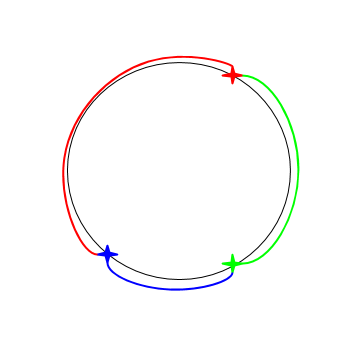
\includegraphics[width=0.3\linewidth]{figs/voro-chord-normal}
		\label{fig:voro-chord-normal}
	\end{figure}
	
\end{frame}
\begin{frame}{Chord Using A Different Closest Metric}
	\begin{figure}
		\centering
		\caption{A Voronoi diagram for a Chord network, where closest if defined by the node being the closest in either direction.}
		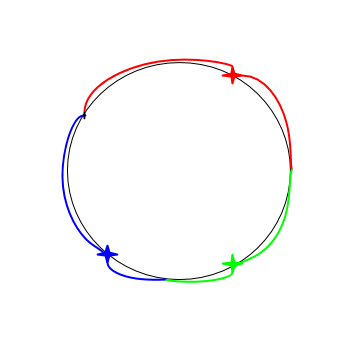
\includegraphics[width=0.5\linewidth]{figs/voro-chord-alternative}
		
		\label{fig:voro-chord-alternative}
	\end{figure}
\end{frame}





\begin{frame}{Terms and Variables}
	\begin{itemize}
		\item Network size is $n$ nodes.
		\item Keys and IDs are generated $m$ bit hash, usually SHA1.
		\item Peerlists are made up of:
		\begin{description}
			\item[Short Peers] The neighboring nodes that define the network's topology.
			\item[Long Peers] Routing shortcuts.
		\end{description}
		\item We'll call the node responsible for a key the $ root $ of the key.
	\end{itemize}
\end{frame}

\note[itemize]{
	\item SHA1 is being depreciated.  
	\item Short peers are actively maintained, long peers replaced gradulally and are not actively pinged.
	\item We use root as it's is a topology agnostic term.
	}






\begin{frame}{Functions}
	\begin{description}
		\item[lookup($ key $)] Finds the node responsible for a given key.
		\item[put($ key $, $ value $)] Stores $value$ at the node responsible for $key$, where $key =  hash(value)$.
		\item[get($ key $)] Returns the $ value $ associated with $key$.
	\end{description}
\end{frame}

\note[itemize]{
	\item There is usually a delete function as well, but it's not important.
	\item All nodes use the same general lookup:  Forward the message to the node closest to $key$
}





\subsection{Chord}

\begin{frame}{Chord}
	\begin{itemize}
		\item Ring Topology
		\item Short Peers: predecessor and successor in the ring.
		\item Responsible for keys between their predecessor and their own.
		\item Long Peers:  $\log n$ nodes, where the node at index $i$ in the  peerlist is 
		$$ root(r + 2^{i-1}) \mod  m,  1 < i  < m $$
		
		
		
	\end{itemize}
\end{frame}

\note[itemize]{
	\item Chord is a favorite because we can draw it.
	\item Draw a Chord network on the wall?
	\item node $r$ is our root node.
	\item $ i $ is the index on the list
	\item English for  the equation, the long peers double in distance from the root node, allowing us to cover at least half the distance to our target in a step
	\item In this way, we can achieve an expected $ \lg n $  hops. 
}

\begin{frame}{A Chord Network}
	\begin{figure}
		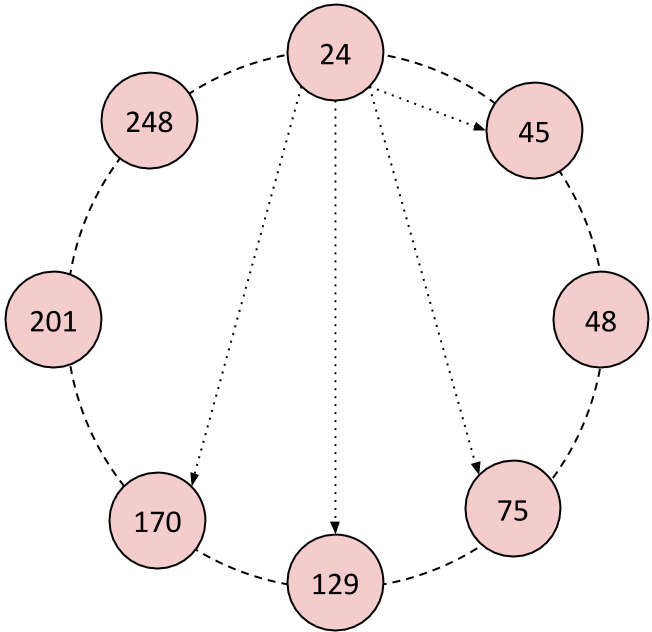
\includegraphics[width=0.55\linewidth]{figs/CR_overlay}
		\caption{An 8-node Chord ring where $m=8$.  Node 24's fingers are shown.}
		\label{fig:chordreal}
	\end{figure}
\end{frame}



\begin{frame}{Fault Tolerence in Chord}
	\begin{itemize}
		\item Local maintenance thread  gradually fixes the network topology.
		\begin{itemize}
			\item Each node ``notifies'' its successor.
			\item The successor replies with a better successor if one exists.
		\end{itemize}
		\item The long peers are gradually updated by performing a lookup on each entry.
		\item Some implementations use predecessor and successor lists.
	\end{itemize}
\end{frame}



\begin{frame}{Handling Churn in General}
	\begin{itemize}
		\item Short peers, the neighbors, are periodically queried to:
		\begin{itemize}
			\item See of the node is still alive.
			\item See if the neighbor knows about better nodes.
		\end{itemize}
		\item Long peer failures are replaced by regular maintenance.
	\end{itemize}
\end{frame}


\subsection{Other DHTs}
\begin{frame}{Other DHTs}
\end{frame}

\section{Completed Work}

\subsection{ChordReduce}

\begin{frame}{ChordReduce}
	content
\end{frame}


\begin{frame}{Churn Results}
	\begin{table}
		\centering
		\begin{tabular}{|r|r|r|} 
			\hline 
			Churn rate per second & Average runtime (s) & Speedup vs 0\% churn\\ \hline{}
			0.8\% & 191.25 & 2.15 \\ \hline
			0.4\% & 329.20 & 1.25 \\ \hline
			0.025\% & 431.86 & 0.95 \\ \hline 
			0.00775\%  & 445.47 & 0.92 \\ \hline 
			0.00250\% & 331.80  &  1.24 \\ \hline 
			0\% & 441.57 & 1.00 \\ \hline
		\end{tabular}
		\caption{The results of calculating $\pi$ by generating $10^8$ samples under churn. Churn is the chance for each node to join or leave the network. The large speedup is from joining nodes acquiring work during experimental runtime.} 
		\label{tab:churnSpeed}
	\end{table}
	
\end{frame}


\subsection{VHash}


\begin{frame}{DHT and Voronoi Relationship}
	\begin{itemize}
	
		\item Most DHTs optimize routing for the number of hops, rather than latency.
		\item We discovered a mapping between Distributed Hash Tables and Voronoi/Delaunay Triangulations.
	\end{itemize}
\end{frame}

\begin{frame}{Voronoi Tesselation}
	\begin{figure}
		\centering
		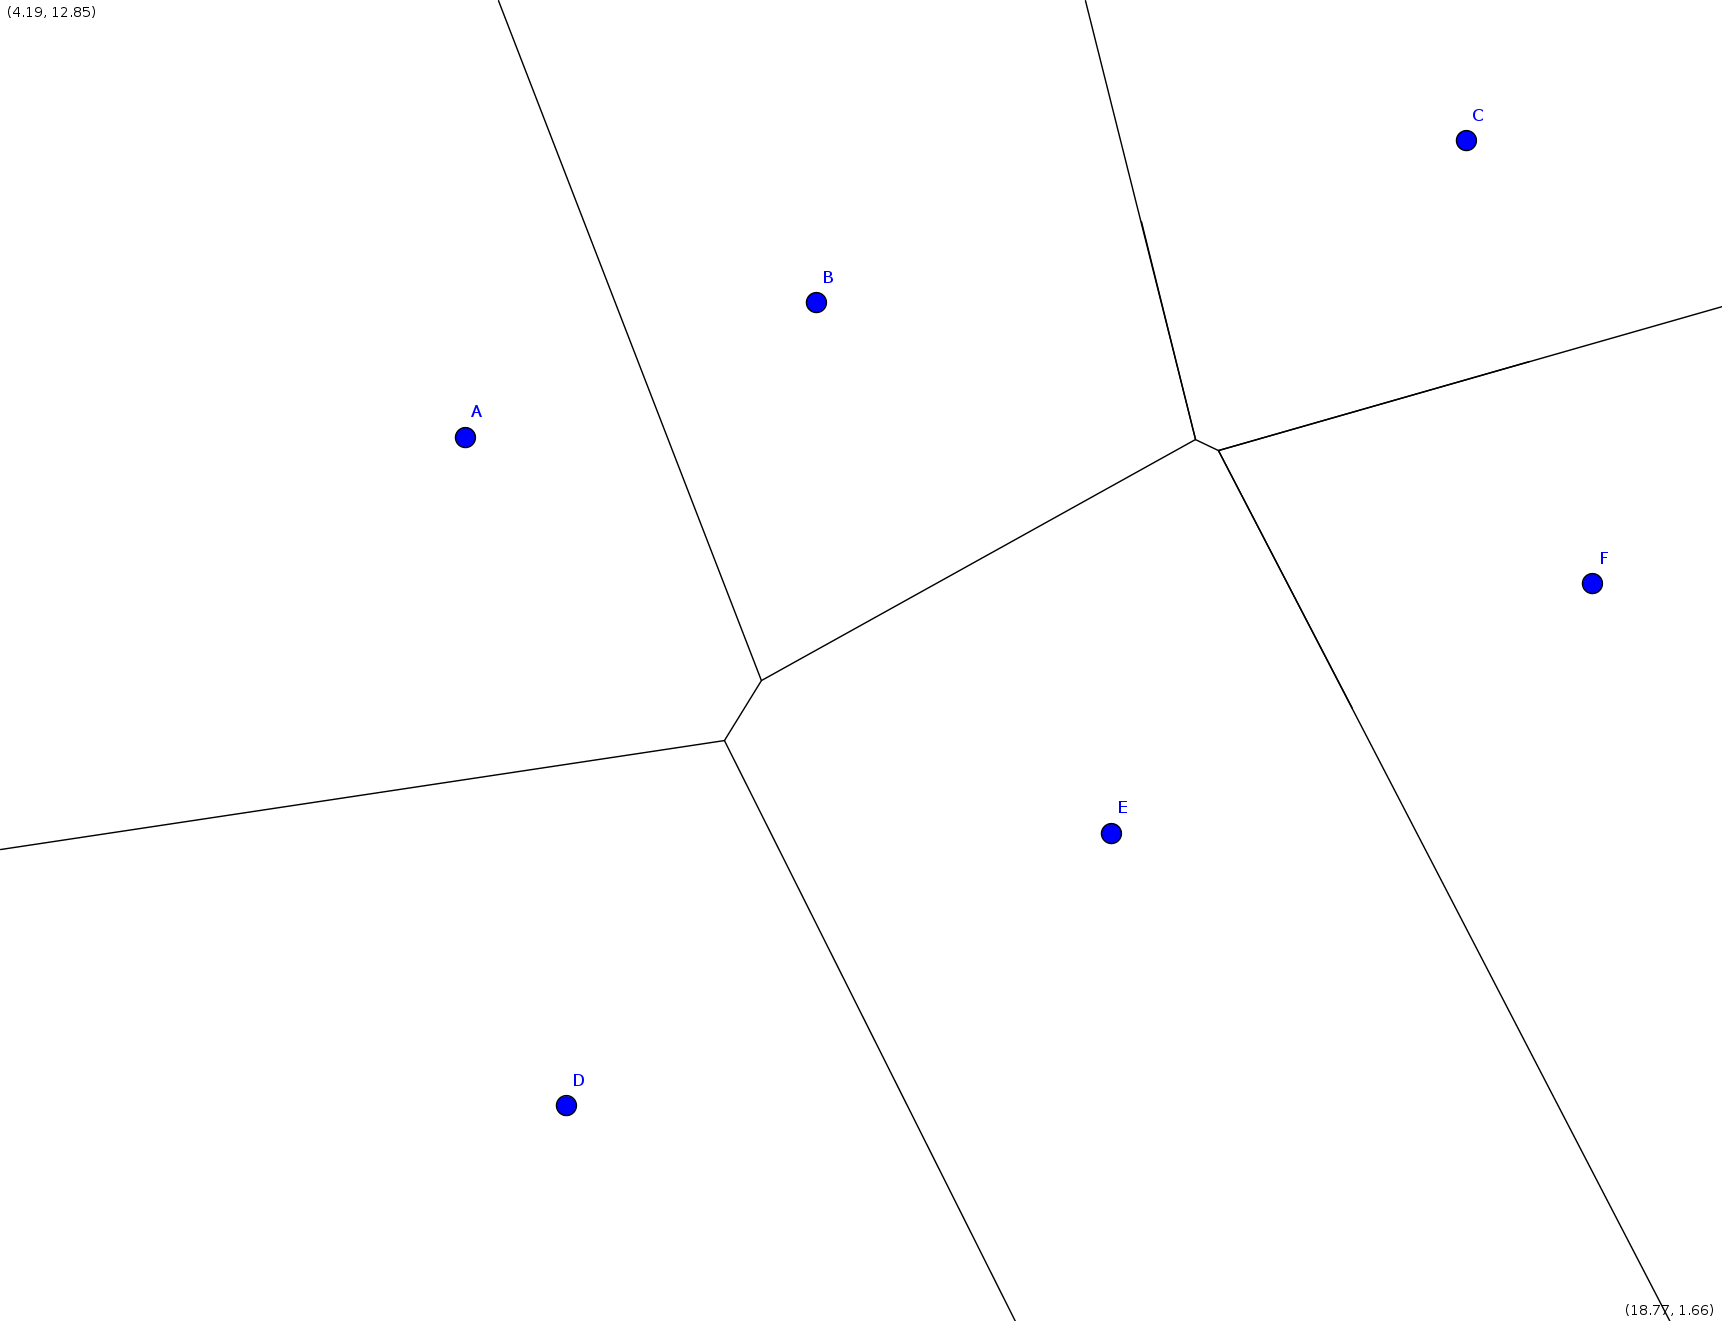
\includegraphics[width=0.5\linewidth]{figs/new_voronoi}
		\caption{A set of points and the generated Voronoi regions}
		\label{fig:new_voronoi}
	\end{figure}
\end{frame}

\note{Define
	\begin{itemize}
		\item Voronoi generators
		\item Voronoi Region
		\item Voronoi Tessellation/ Diagram
	\end{itemize}
}

\begin{frame}{Delaunay Triangulation}
	\begin{figure}
		\centering
		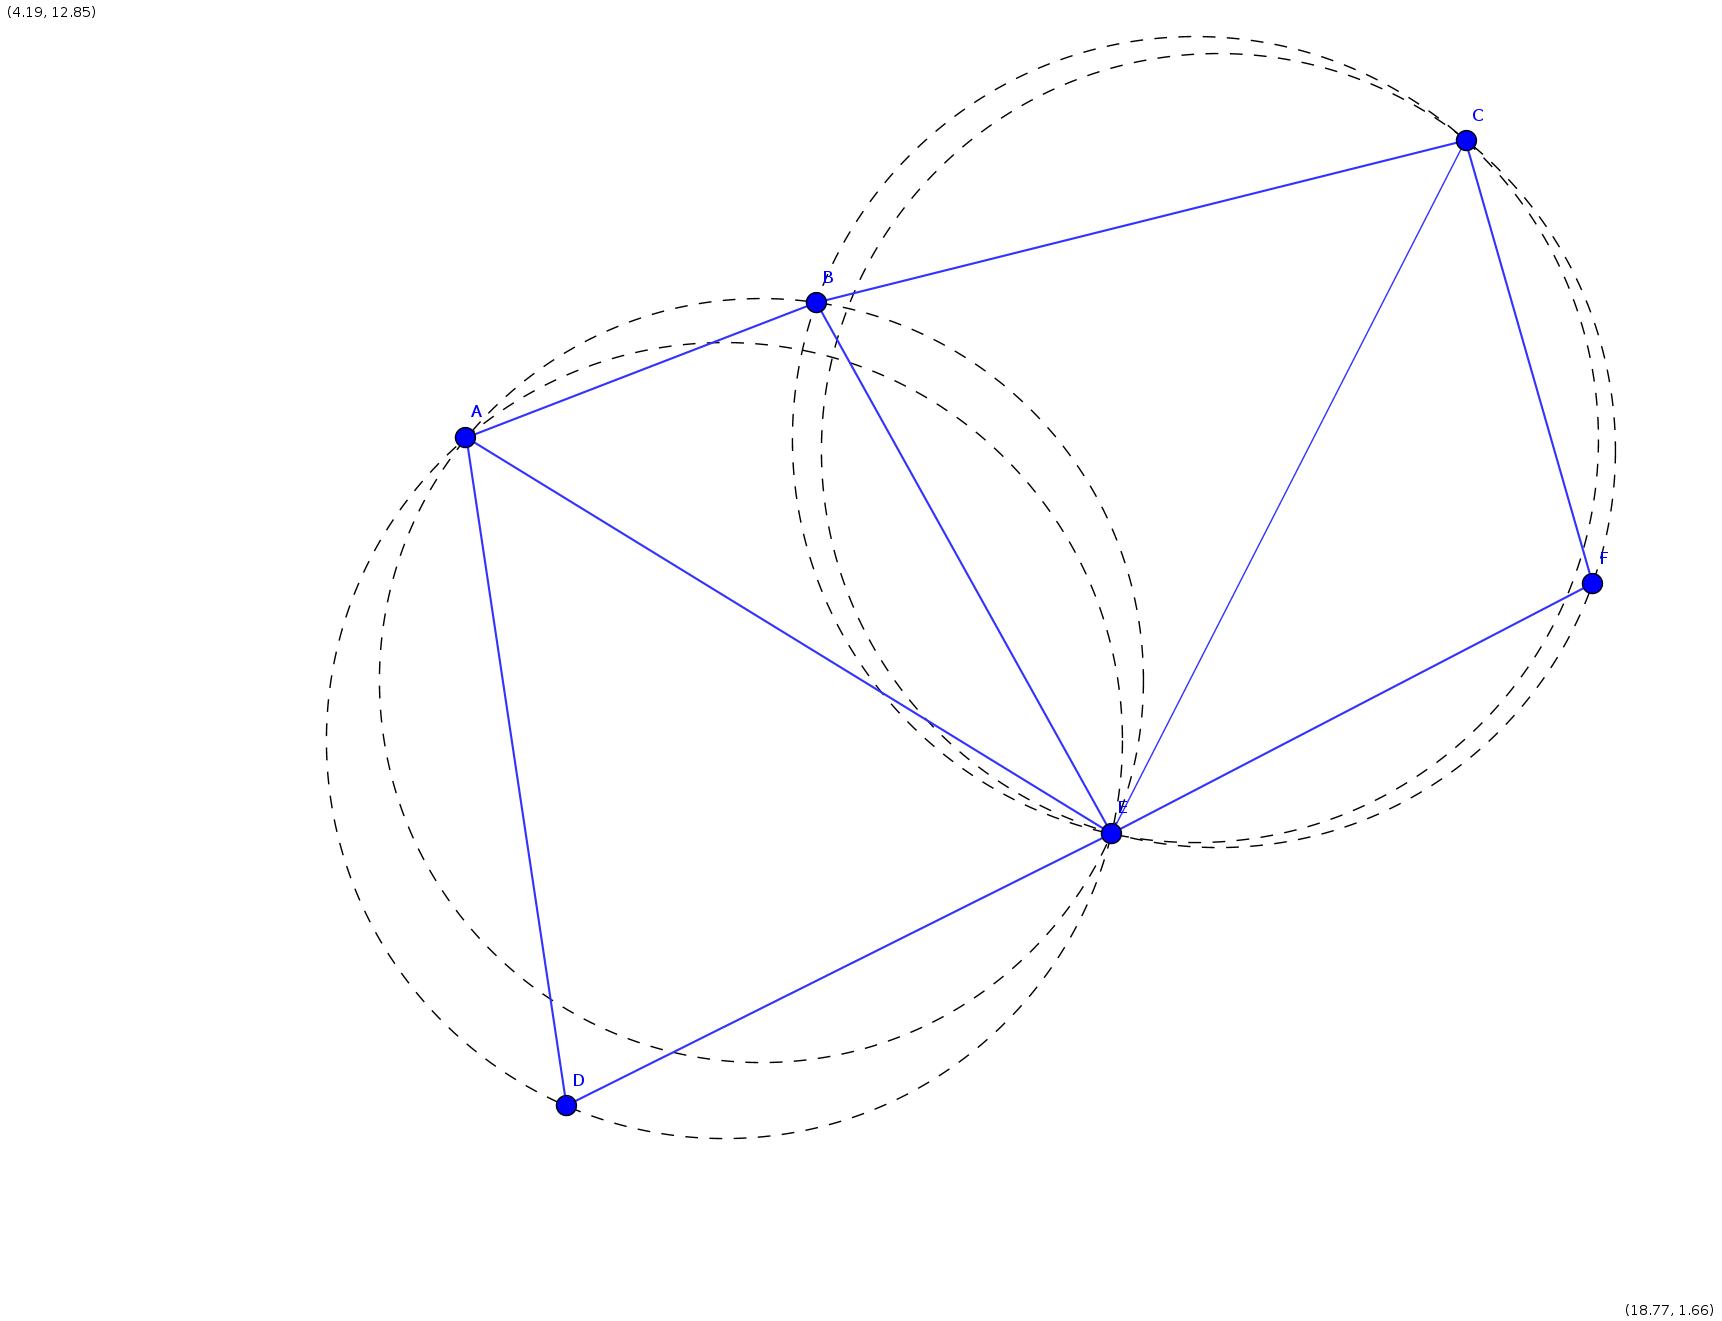
\includegraphics[width=0.5\linewidth]{figs/delaunay}
		\caption{The same set of nodes with their corresponding Delaunay Triangulation.}
		\label{fig:delaunay}
	\end{figure}
\end{frame}


\begin{frame}{DHT and Voronoi Relationship }
	\begin{itemize}
		\item Coprime
		\item We can view DHTs in terms of Voronoi and Delaunay
		\begin{itemize}
			\item The set of keys the node is responsible for is its Voronoi region.
			\item The nodes neighbors are it's Delaunay neighbors.
		\end{itemize}
	\end{itemize}
\end{frame}

\begin{frame}{VHash}
	\begin{itemize}
		\item Voronoi-based Distributed Hash Table
	\end{itemize}
\end{frame}


\begin{frame}{DGVH}
	content
\end{frame}






\begin{frame}{Results}
	\begin{figure}
		\centering
		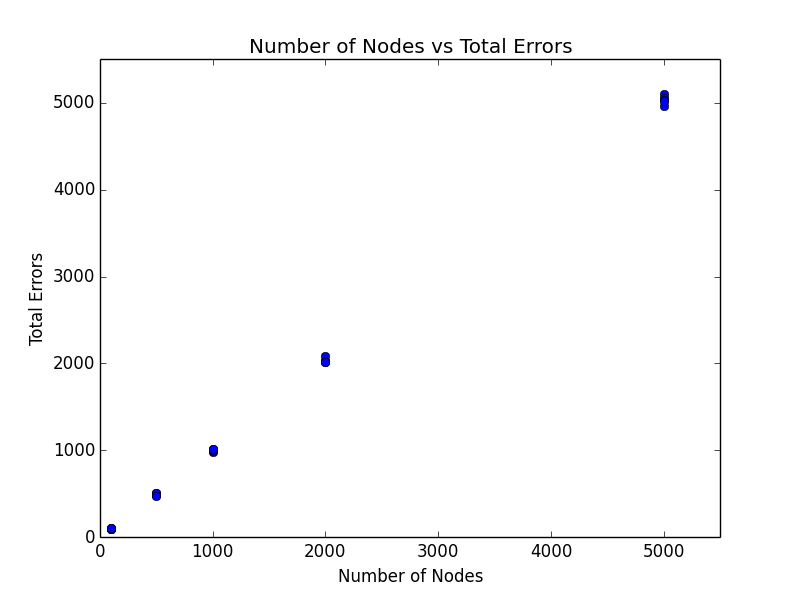
\includegraphics[width=0.5\linewidth]{figs/error_rate}
		\caption{As the size of the graph increases, we see approximately 1 error per node.
		We can also see that the error rate and number of nodes has a linear relationship.}
		\label{exp_0}
	\end{figure}
\end{frame}


\begin{frame}{Results}
	\begin{figure}
		\label{fig:conv}
		\begin{subfigure}[b]{.45\linewidth}
			\centering
			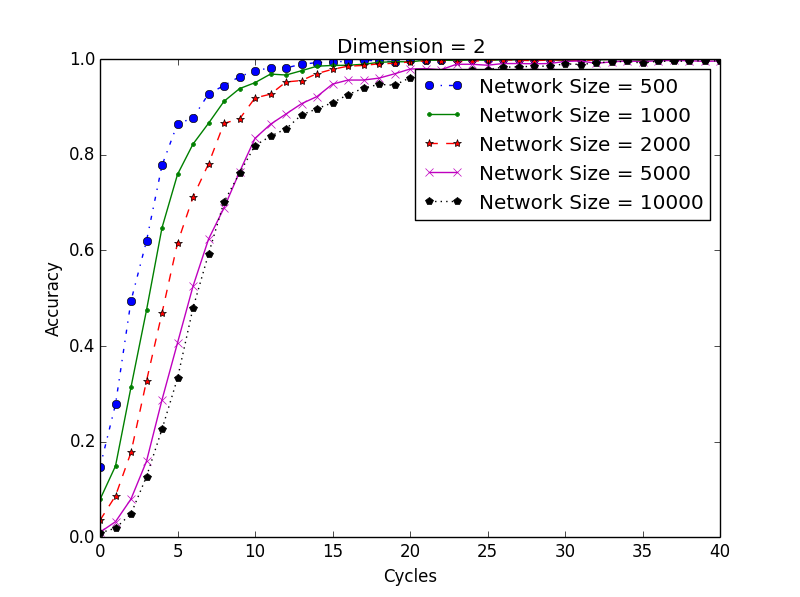
\includegraphics[height=3cm]{figs/conv_d2}
			%\caption{This plot shows the accuracy rate of lookups on a 2-dimensional network as it self-organizes.}
			\label{conv2}
		\end{subfigure} 
		\begin{subfigure}[b]{.45\linewidth}
			\centering
			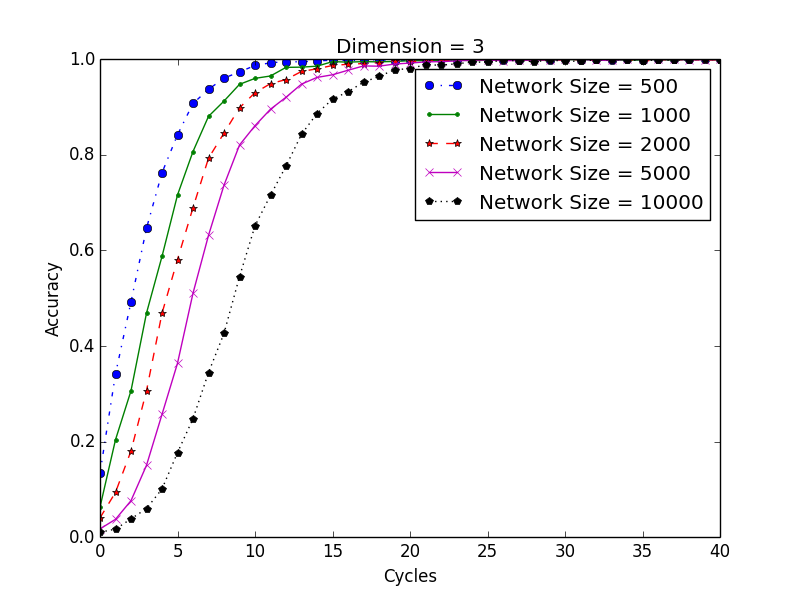
\includegraphics[height=3cm]{figs/conv_d3}
			%\caption{This plot shows the accuracy rate of lookups on a 3-dimensional network as it self-organizes.}
			\label{conv3}
		\end{subfigure}\\
		\begin{subfigure}[b]{.45\linewidth}
			\centering
			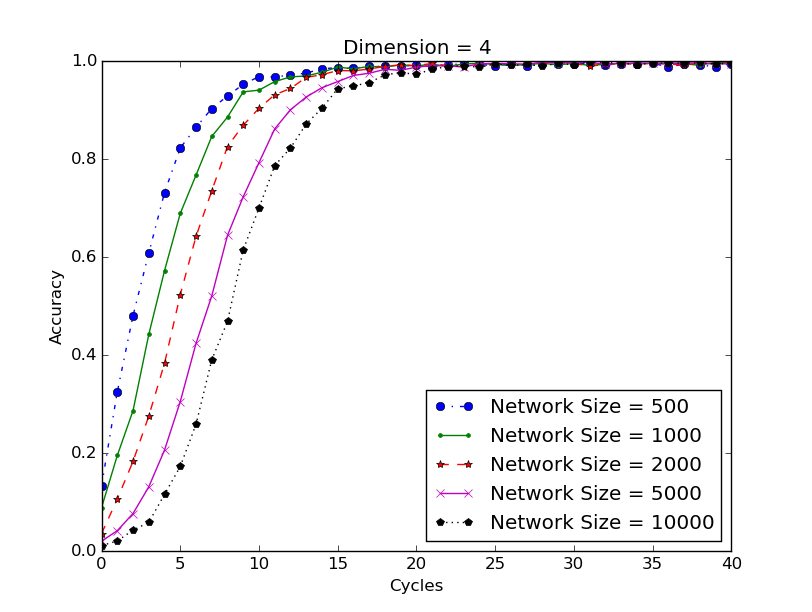
\includegraphics[height=3cm]{figs/conv_d4}
			%\caption{This plot shows the accuracy rate of lookups on a 4-dimensional network as it self-organizes.}
			\label{conv4}
		\end{subfigure}
		\begin{subfigure}[b]{.45\linewidth}
			\centering
			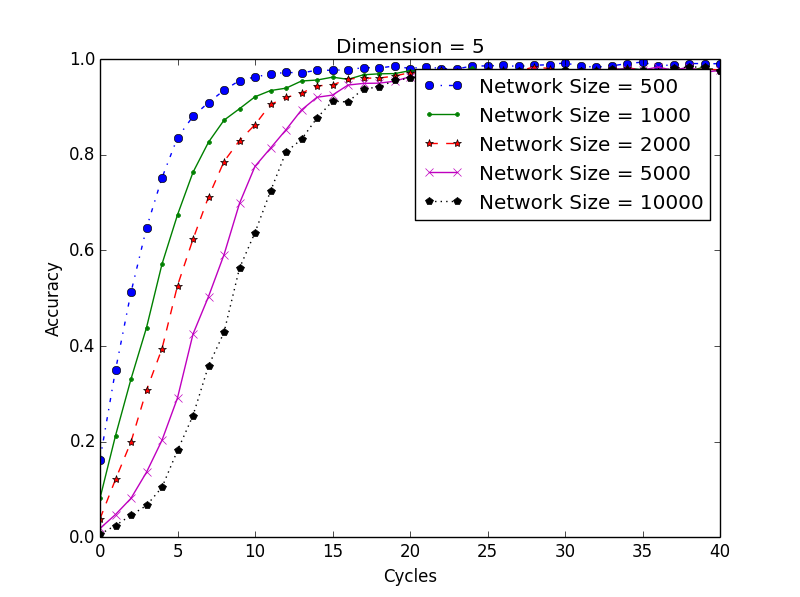
\includegraphics[height=3cm]{figs/conv_d5}
			%\caption{This plot shows the accuracy rate of lookups on a 5-dimensional network as it self-organizes.}
			\label{conv5}
		\end{subfigure}
		
		\caption{These figures show, starting from a randomized network, VHash forms a stable and consistent network topology. %The Y axis is the percentage of successful lookups out of 2000 queries and the X axis is the number of gossips cycles.}
		}
		
	\end{figure}
\end{frame}

\subsection{Sybil Attack Analysis}

\begin{frame}{The Sybil Attack}
	\begin{itemize}
		\item The 
	\end{itemize}
\end{frame}



\begin{frame}
	\frametitle{The goal of the Sybil Attack in A P2P network}
	See Whiteboard
	\begin{itemize}
		\item We want to inject a Sybil into as many of the regions between nodes as we can.
		\item The question I wanted to answer is what is the probability that a region can have a Sybil injected into it, given:
		\begin{itemize}
			\item The network size $n$
			\item The number of keys (IDs) available to the attacker (the number of identities they can fake).
		\end{itemize}
	\end{itemize}
	\end{frame} 
       
\begin{frame}
\frametitle{Assumptions}
	\begin{itemize}
		\item The attacker is limited in the number of identities they can fake.
		
		\begin{itemize}
			\item To fake an identity, the attacker must be able to generate a valid IP/port combo he owns.
			\item The attacker therefore has $num\_IP \cdot num\_ports$ IDs.
			\item We'll set $ num\_ports = 16383 $, the number of ephemeral ports.
			\item Storage cost is 320 KiB.
		\end{itemize}
		\item We call the act of finding an ID by modulating your IP and port so you can inject a node \emph{mashing}.
		\item In Mainline DHT, used by BitTorrent, you can choose your own ID at ``random.''   The implications should be apparent.
	
	\end{itemize}
\end{frame}

\begin{frame}
    \frametitle{Analysis}
    The probability you can mash a region between two adjacent nodes in a size $n$ network is:
     \begin{equation}
    P \approx \frac{1}{n}\cdot num\_ips \cdot num\_ports
    \end{equation}
    An attacker can compromise a portion $ P_{bad\_neighbor} $ of the network given by:
    \begin{equation}
    P_{bad\_neighbor} =  \frac{num\_ips \cdot num\_ports}{num\_ips \cdot num\_ports + n - 1}
    \label{eq:bad}
    \end{equation}
    
\end{frame}
\note[itemize]{\item Have proofs!}


\subsubsection{Results}

\begin{frame}
    \begin{figure}
        \centering
        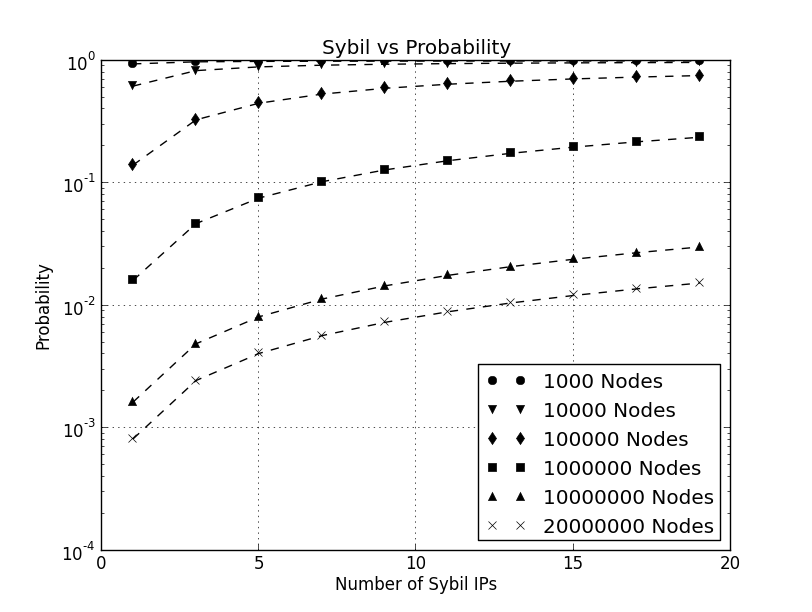
\includegraphics[width=0.65\linewidth]{figs/ip_prob_all}
        \caption[foo]{Our simulation results.  
            The $x$-axis corresponds to the number of IP addresses the adversary can bring to bear.
            The $y$-axis is the probability that a random region between two adjacent normal members of the network can be mashed.
            Each line maps to a different network size of $n$.
            The dotted line traces the line corresponding to the Equation \ref{eq:bad}: $ P_{bad\_neighbor} =  \frac{num\_ips \cdot 16383}{num\_ips \cdot 16383 + n - 1}$}.
        \label{fig:exp2}
    \end{figure}
\end{frame}

\begin{frame}
    
    \begin{figure}
        \centering
        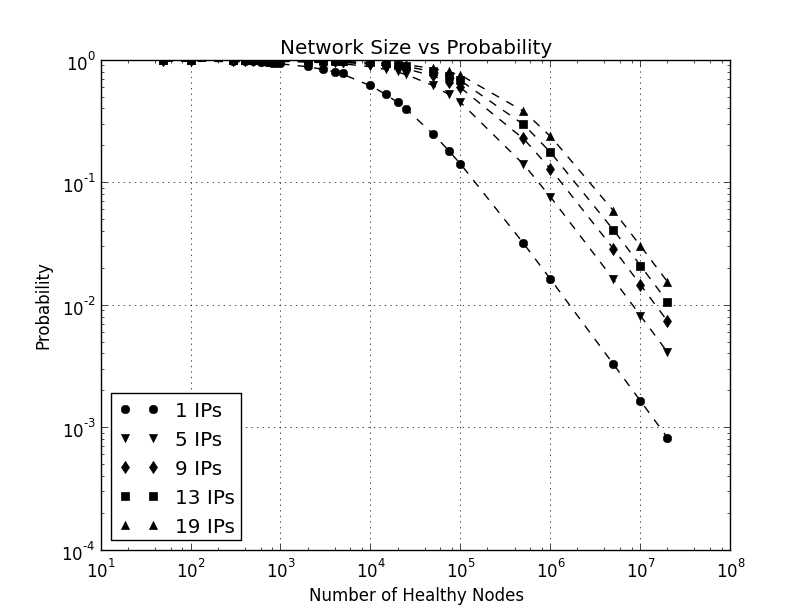
\includegraphics[width=0.7\linewidth]{figs/size_prob_all}
        \caption[a]{These are the same as results shown in Figure \ref{fig:exp2}, but our $x$-axis is the network size $n$ in this case.  
            Here, each line corresponds to a different number of unique IP addresses the adversary has at their disposal.}
        \label{fig:size_prob_all}
    \end{figure}
\end{frame}

\begin{frame}
    \begin{figure}
        \centering
        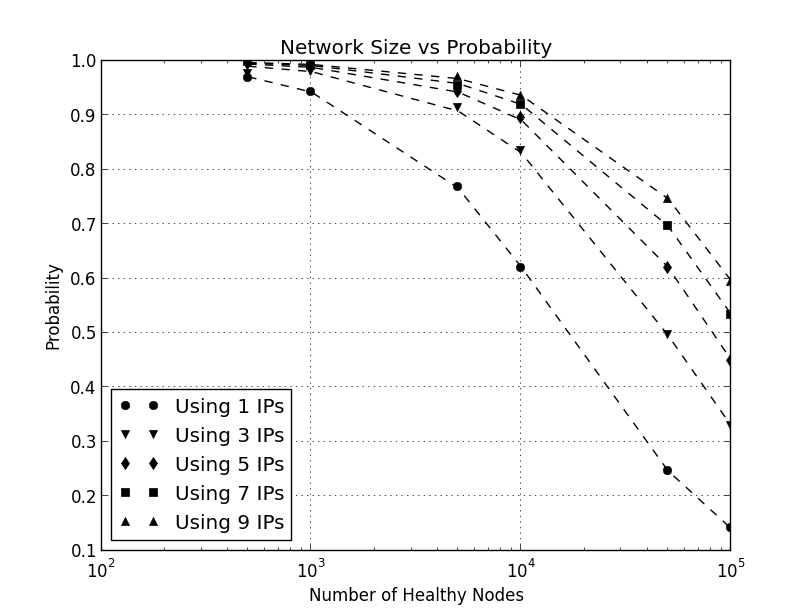
\includegraphics[width=0.7\linewidth]{figs/size_occlusion_chord}
        \caption{This graph shows the relationship between the network size and the probability a particular link, adjacent or not, can be mashed.}
        \label{fig:exp3}
    \end{figure}
\end{frame}
    

\section{Proposed Work}



\subsection{UrDHT}
\begin{frame}{UrDHT}
	This kind of framework does not exist.
	
	VHash is a precursor to this work.
\end{frame}

\note{At Brendan's suggestion We plan on extending the functionality of DHTs, post poll}


\subsection{DHT Distributed Computing}
\begin{frame}{DHT Distributed Computing}
	content
\end{frame}



\subsection{Autonomous Load-Balancing}
\begin{frame}{Autonomous Load-Balancing}
	content
\end{frame}


\bibliography{notes,dht,mapreduce,voronoi,dns,botnets,mine}
\bibliographystyle{plain}
\end{document}
